
% This LaTeX was auto-generated from MATLAB code.
% To make changes, update the MATLAB code and republish this document.

\documentclass{article}
\usepackage{graphicx}
\usepackage{color}
\usepackage{multicol}
\usepackage[a4paper, total={6in, 8in}]{geometry}

\sloppy
\definecolor{lightgray}{gray}{0.5}
\setlength{\parindent}{0pt}

\begin{document}


%=========================================
\hrulefill
\subsection*{Question 1}

%-----------------------------------------
\hrulefill
\subsection*{\#1(a)}

\begin{verbatim}
clear;clc;close all
fun1 = @(n) (-3/5)^(n-1);
x1 = limsum(fun1, 1);
\end{verbatim}

\dotfill
\color{lightgray}
\begin{verbatim}
Iteration times: 29
Value: 0.625000
Error: 0.000001
\end{verbatim}
\color{black}

%-----------------------------------------
\hrulefill
\subsection*{\#1(b)}

\begin{verbatim}
clear;clc;close all
fun2 = @(n) (4/9)^(n-1);
x2 = limsum(fun2, 1);
\end{verbatim}

\dotfill
\color{lightgray}
\begin{verbatim}
Iteration times: 19
Value: 1.800000
Error: 0.000000
\end{verbatim}
\color{black}

%-----------------------------------------
\hrulefill
\subsection*{\#1(c)}

\begin{verbatim}
clear;clc;close all
fun3 = @(n) sin(n*pi()/2)/n;
x3 = limsum(fun3, 1);
\end{verbatim}

\dotfill
\color{lightgray}
\begin{verbatim}
Iteration times: 2
Value: 1.000000
Error: 0.000000
\end{verbatim}
\color{black}

%-----------------------------------------
\hrulefill
\subsection*{\#1(d)}

\begin{verbatim}
clear;clc;close all
sum = 1;
n = 1;
x = [];
while 1
    error = 1;
    for i = 1:2:2*n
        error = error*(i/(i+1));
    end
    error = (-1)^n*(1+4*n)*error^3;
    sum = sum + error;
    if abs(error) < 1e-3
        break
    end
    n = n+1;
end
fprintf("Iteration times: %d \nValue: %f \nError: %f\n\n", n, sum, error);
\end{verbatim}

\dotfill
\color{lightgray}
\begin{verbatim}
Iteration times: 516025
Value: 0.636120
Error: -0.001000
\end{verbatim}
\color{black}

%=========================================
\hrulefill
\subsection*{Question 2}

%-----------------------------------------
\hrulefill
\subsection*{\#2(a)}

\begin{verbatim}
clear;clc;close all
z = 0:0.0001:20;
J0 = besselj(0,z);
plot(z,J0)
grid()
title("Zero order of Bessel function")

roots_ans = [];
count = 0;
for i = 1:length(J0)-1
    if J0(i)*J0(i+1)<0
        count = count+1;
        roots_ans(count) = i;
    end
end
for i = 1:3
    fprintf("lambda%d = %.4f\n",i,z(roots_ans(i)))
end
\end{verbatim}

\dotfill
\color{lightgray}
\begin{verbatim}
lambda1 = 2.4048
lambda2 = 5.5200
lambda3 = 8.6537
\end{verbatim}
\color{black}

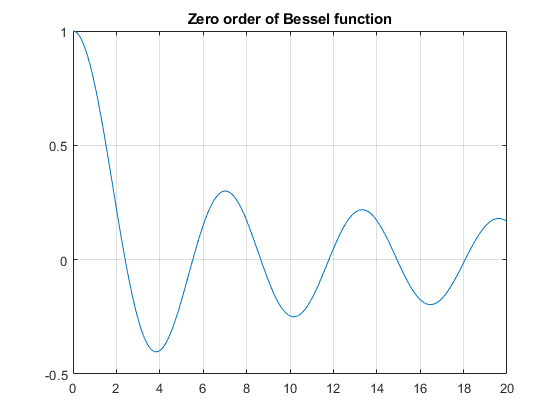
\includegraphics [width=3in]{HW1_01.png}

%-----------------------------------------
\hrulefill
\subsection*{\#2(b)}

\begin{verbatim}
clear;clc;close all
lambda = 0:0.01:400;
y1 = tan(sqrt(lambda)*log(2)/2);
y2 = tan(sqrt(lambda)*log(2));
error = abs(y1-y2);
count = 1;
for i = 1:length(error)
   if error(i) <= 5e-5
       fprintf("lambda_%d = %f\n", count, lambda(i))
       count = count+1;
       figure()
       if i-100 <= 0
           plot(lambda(i:i+100),y1(i:i+100),lambda(i:i+100),y2(i:i+100))
       else
           plot(lambda(i-100:i+100),y1(i-100:i+100),lambda(i-100:i+100),y2(i-100:i+100))
       end
       legend('y1','y2')
   end
end
\end{verbatim}

\newpage
\dotfill
\color{lightgray}
\begin{verbatim}
lambda_1 = 0.000000
lambda_2 = 82.170000
lambda_3 = 328.680000
\end{verbatim}
\color{black}

\begin{multicols}{3}
    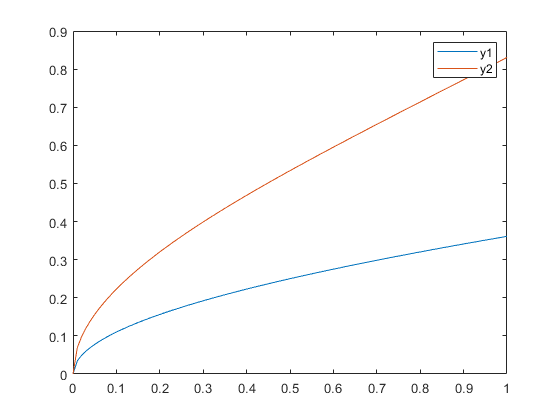
\includegraphics [width=2in]{HW1_02.png}

    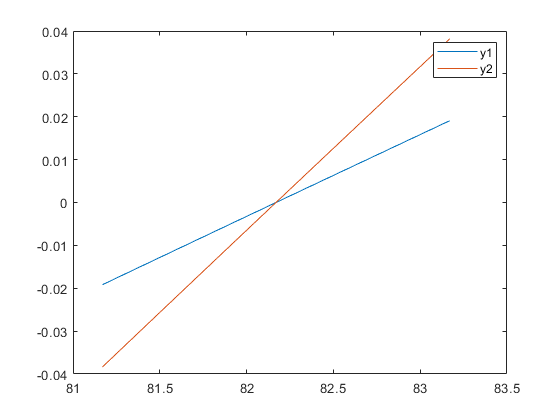
\includegraphics [width=2in]{HW1_03.png}

    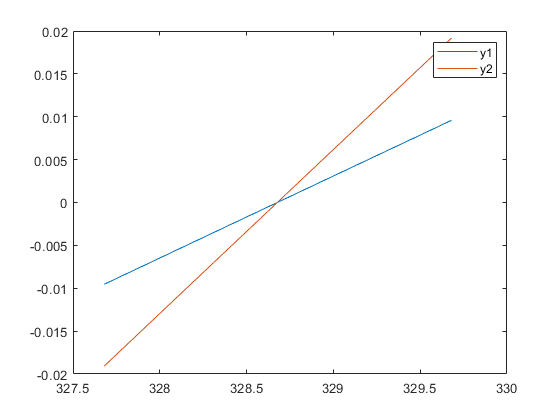
\includegraphics [width=2in]{HW1_04.png}
\end{multicols}

%=========================================
\hrulefill
\subsection*{Question 3}

%-----------------------------------------
\hrulefill
\subsection*{\#3(a)}

\begin{verbatim}
clear;clc;close all
[x, y] = meshgrid(-4:0.1:4);
T = y./(x.^2+y.^2);
figure()
surf(x,y,T)
title("$\frac{y}{x^2+y^2}$ 3D Plot",'FontSize',15,'interpreter','latex')

figure()
contour(x,y,T, 30,'ShowText','on')
title("$\frac{y}{x^2+y^2}$ 2D Plot",'FontSize',15,'interpreter','latex')
\end{verbatim}

\dotfill\\
\newpage
\begin{multicols}{2}
    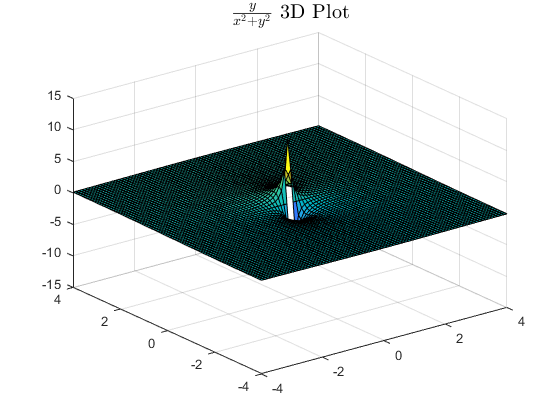
\includegraphics [width=3in]{HW1_05.png}

    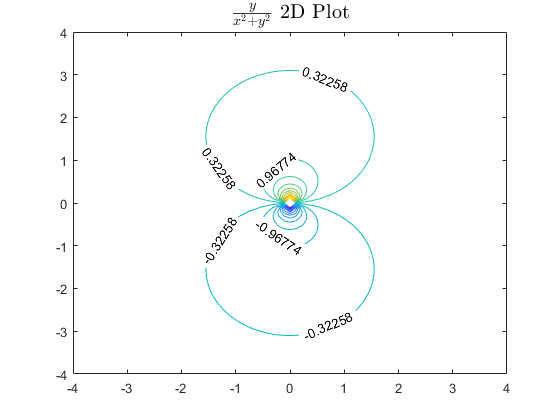
\includegraphics [width=3in]{HW1_06.png}
\end{multicols}

%-----------------------------------------
\hrulefill
\subsection*{\#3(b)}

\begin{verbatim}
clear;clc;close all
[x, y] = meshgrid(-10:0.1:10);
T = log(x.^2+y.^2);
figure()
surf(x,y,T)
title("$\ln(x^2+y^2)$ 3D Plot",'FontSize',15,'interpreter','latex')

figure()
contour(x,y,T,'ShowText','on')
title("$\ln(x^2+y^2)$ 2D Plot",'FontSize',15,'interpreter','latex')
\end{verbatim}

\dotfill\\
\begin{multicols}{2}
    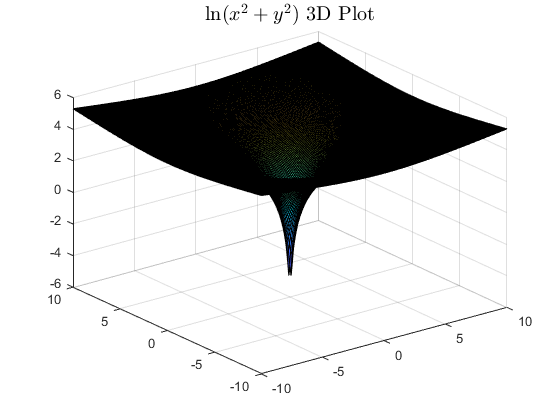
\includegraphics [width=3in]{HW1_07.png}

    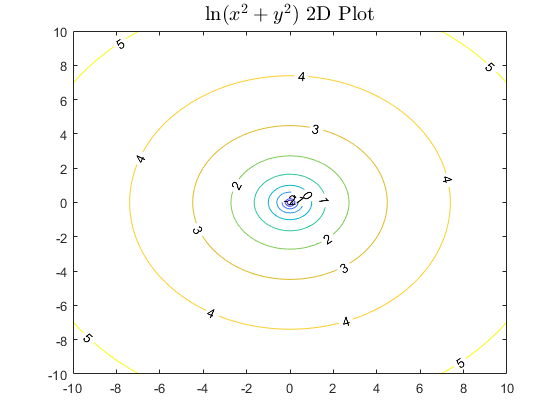
\includegraphics [width=3in]{HW1_08.png}
\end{multicols}

%-----------------------------------------
\hrulefill
\subsection*{\#3(c)}

\begin{verbatim}
clear;clc;close all
[x, y] = meshgrid(0:0.1:10,0:0.1:pi());
len = size(x);
for i = 1:len(1)
    for j = 1:len(2)
        f = @(n) exp(-(2.*n-1).*x(i,j)).*sin((2.*n-1).*y(i,j))./(2.*n-1);
        T(i,j) = 4*limsum(f,0)/pi();
    end
end
figure()
surf(x,y,T)
title("$\frac{4}{\pi}\sum_{n=1,3,5,...}^{\infty}\frac{1}{n}\exp^{-nx}\sin{ny}$ 3D Plot",...
'FontSize',15,'interpreter','latex')

figure()
contour(x,y,T,'ShowText','on')
title("$\frac{4}{\pi}\sum_{n=1,3,5,...}^{\infty}\frac{1}{n}\exp^{-nx}\sin{ny}$ 2D Plot",...
'FontSize',15,'interpreter','latex')
\end{verbatim}

\dotfill\\
\begin{multicols}{2}
    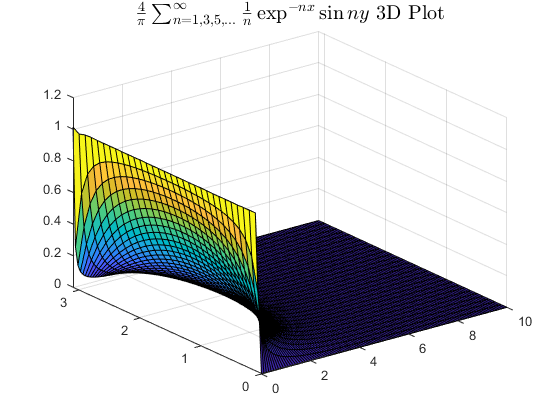
\includegraphics [width=3in]{HW1_09.png}

    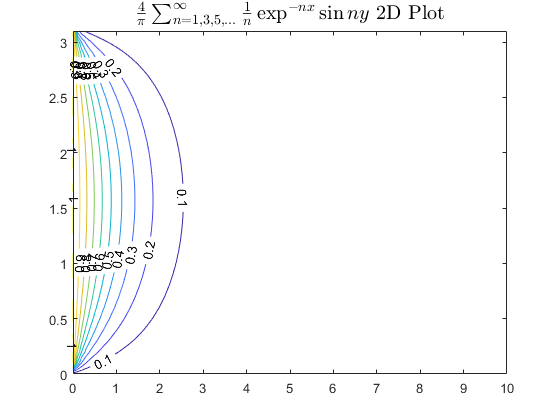
\includegraphics [width=3in]{HW1_10.png}
\end{multicols}

%-----------------------------------------
\hrulefill
\subsection*{\#3(d)}

\begin{verbatim}
clear;clc;close all
[x, y] = meshgrid(0:0.1:10,0:0.1:pi());
T = 2.*atan2(sin(y),sinh(x))./pi();
figure()
surf(x,y,T)
title("$\frac{2}{\pi}\tan^{-1}{(\frac{\sin{y}}{\sinh{x}})}$ 3D Plot",...
'FontSize',15,'interpreter','latex')

figure()
contour(x,y,T,'ShowText','on')
title("$\ln(x^2+y^2)$ 2D Plot",'FontSize',15,'interpreter','latex')
\end{verbatim}

\dotfill\\
\begin{multicols}{2}
    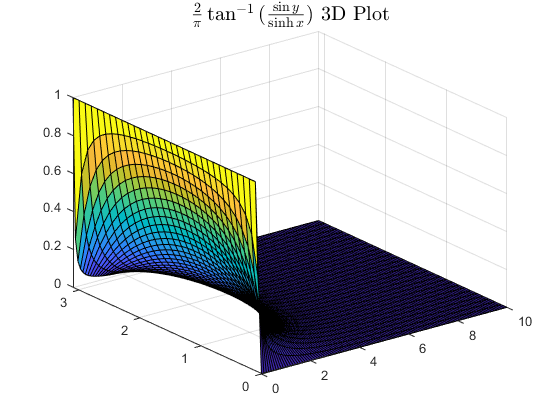
\includegraphics [width=3in]{HW1_11.png}

    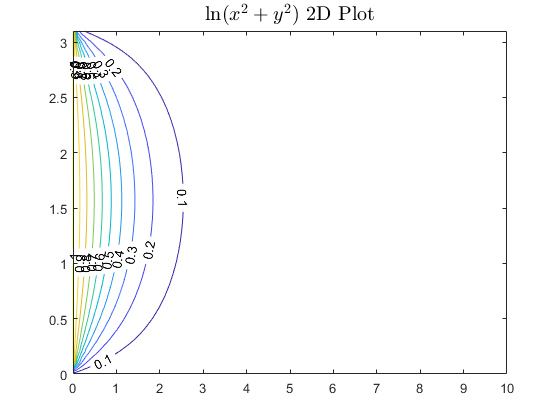
\includegraphics [width=3in]{HW1_12.png}
\end{multicols}

%=========================================
\hrulefill
\subsection*{Question 4}

%-----------------------------------------
\hrulefill
\subsection*{\#4(a)}

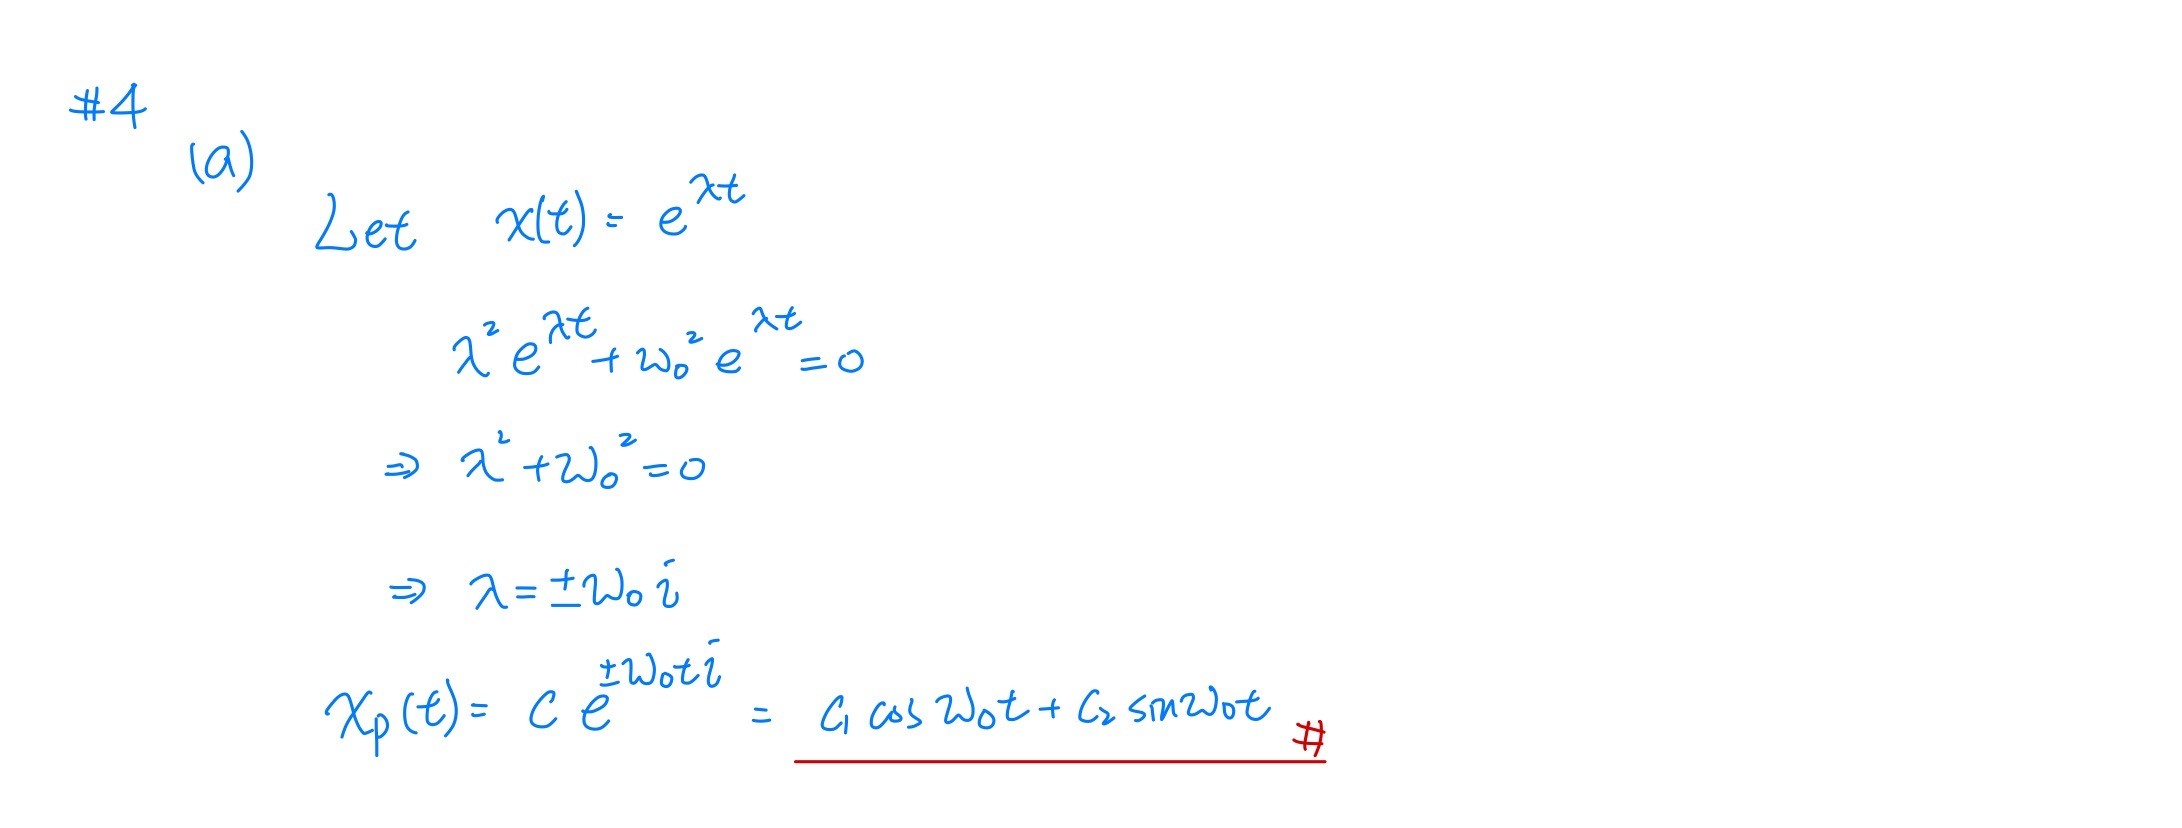
\includegraphics[width=6in]{4(a).jpg}

%-----------------------------------------
\hrulefill
\subsection*{\#4(b)(1)}

\begin{verbatim}
clear;clc;close all
t = 0:0.01:50;
x = sin(t./4);
plot(t,x)
grid()
title("$\sin{\frac{t}{4}}$",'FontSize',15,'interpreter','latex')
\end{verbatim}

\dotfill\\
\\
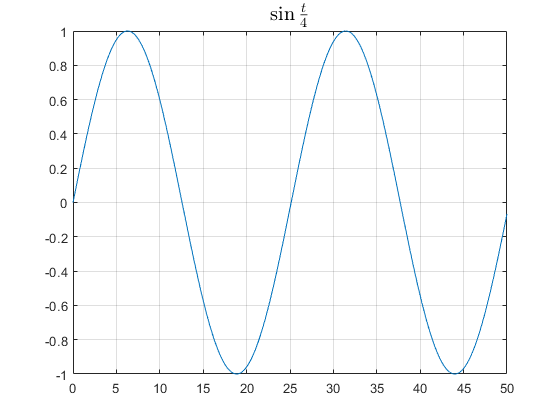
\includegraphics [width=3in]{HW1_13.png}

%-----------------------------------------
\hrulefill
\subsection*{\#4(b)(2)}

\begin{verbatim}
clear;clc;close all
t = 0:0.01:50;
x = sin(5.*t./2);
plot(t,x)
grid()
title("$\sin{\frac{5t}{2}}$",'FontSize',15,'interpreter','latex')
\end{verbatim}

\dotfill\\
\\
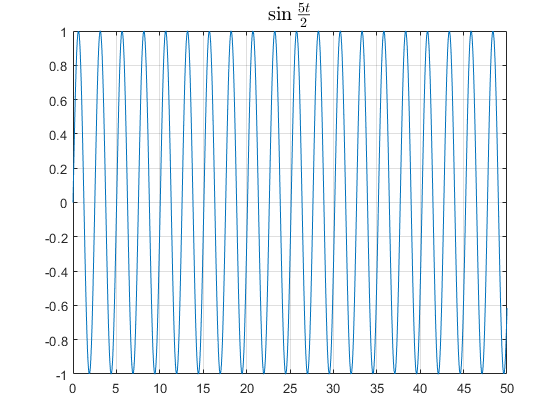
\includegraphics [width=3in]{HW1_14.png}

%-----------------------------------------
\hrulefill
\subsection*{\#4(b)(3)}

\begin{verbatim}
clear;clc;close all
t = 0:0.01:50;
x = sin(t./4).*sin(5.*t./2);
plot(t,x)
grid()
title("$\sin{\frac{t}{4}}\sin{\frac{5t}{2}}$",'FontSize',15,'interpreter','latex')
\end{verbatim}

\dotfill\\
\\
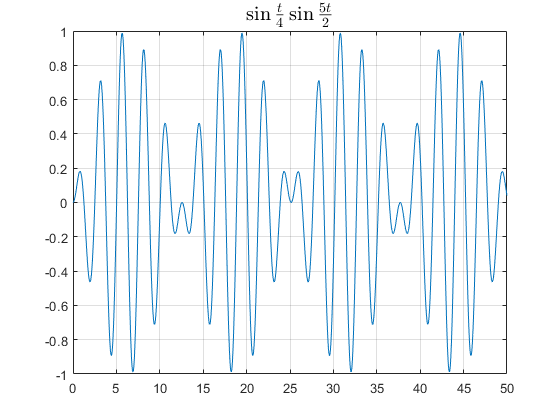
\includegraphics [width=3in]{HW1_15.png}

%-----------------------------------------
\hrulefill
\subsection*{\#4(c)}

\begin{verbatim}
clear;clc;close all
global w0 omega
w0 = 1;
omega = 1;
[t, x] = ode45(@vibration_eqn, [0 10], [0; 0]);
plot(t,x)
legend('x','dx/dt')
grid()
title("")
\end{verbatim}

\dotfill\\
\\
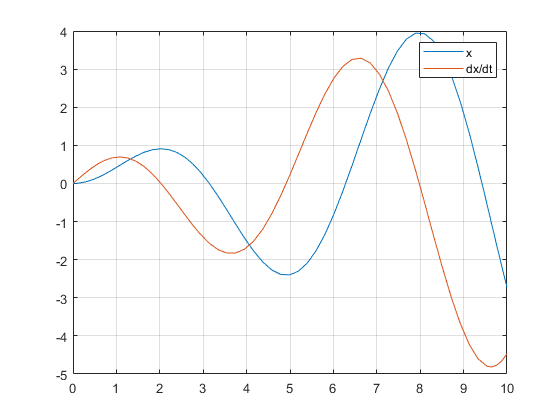
\includegraphics [width=3in]{HW1_16.png}

%=========================================
\newpage
\hrulefill
\subsection*{Question 5}

%-----------------------------------------
\hrulefill
\subsection*{\#5(a)}

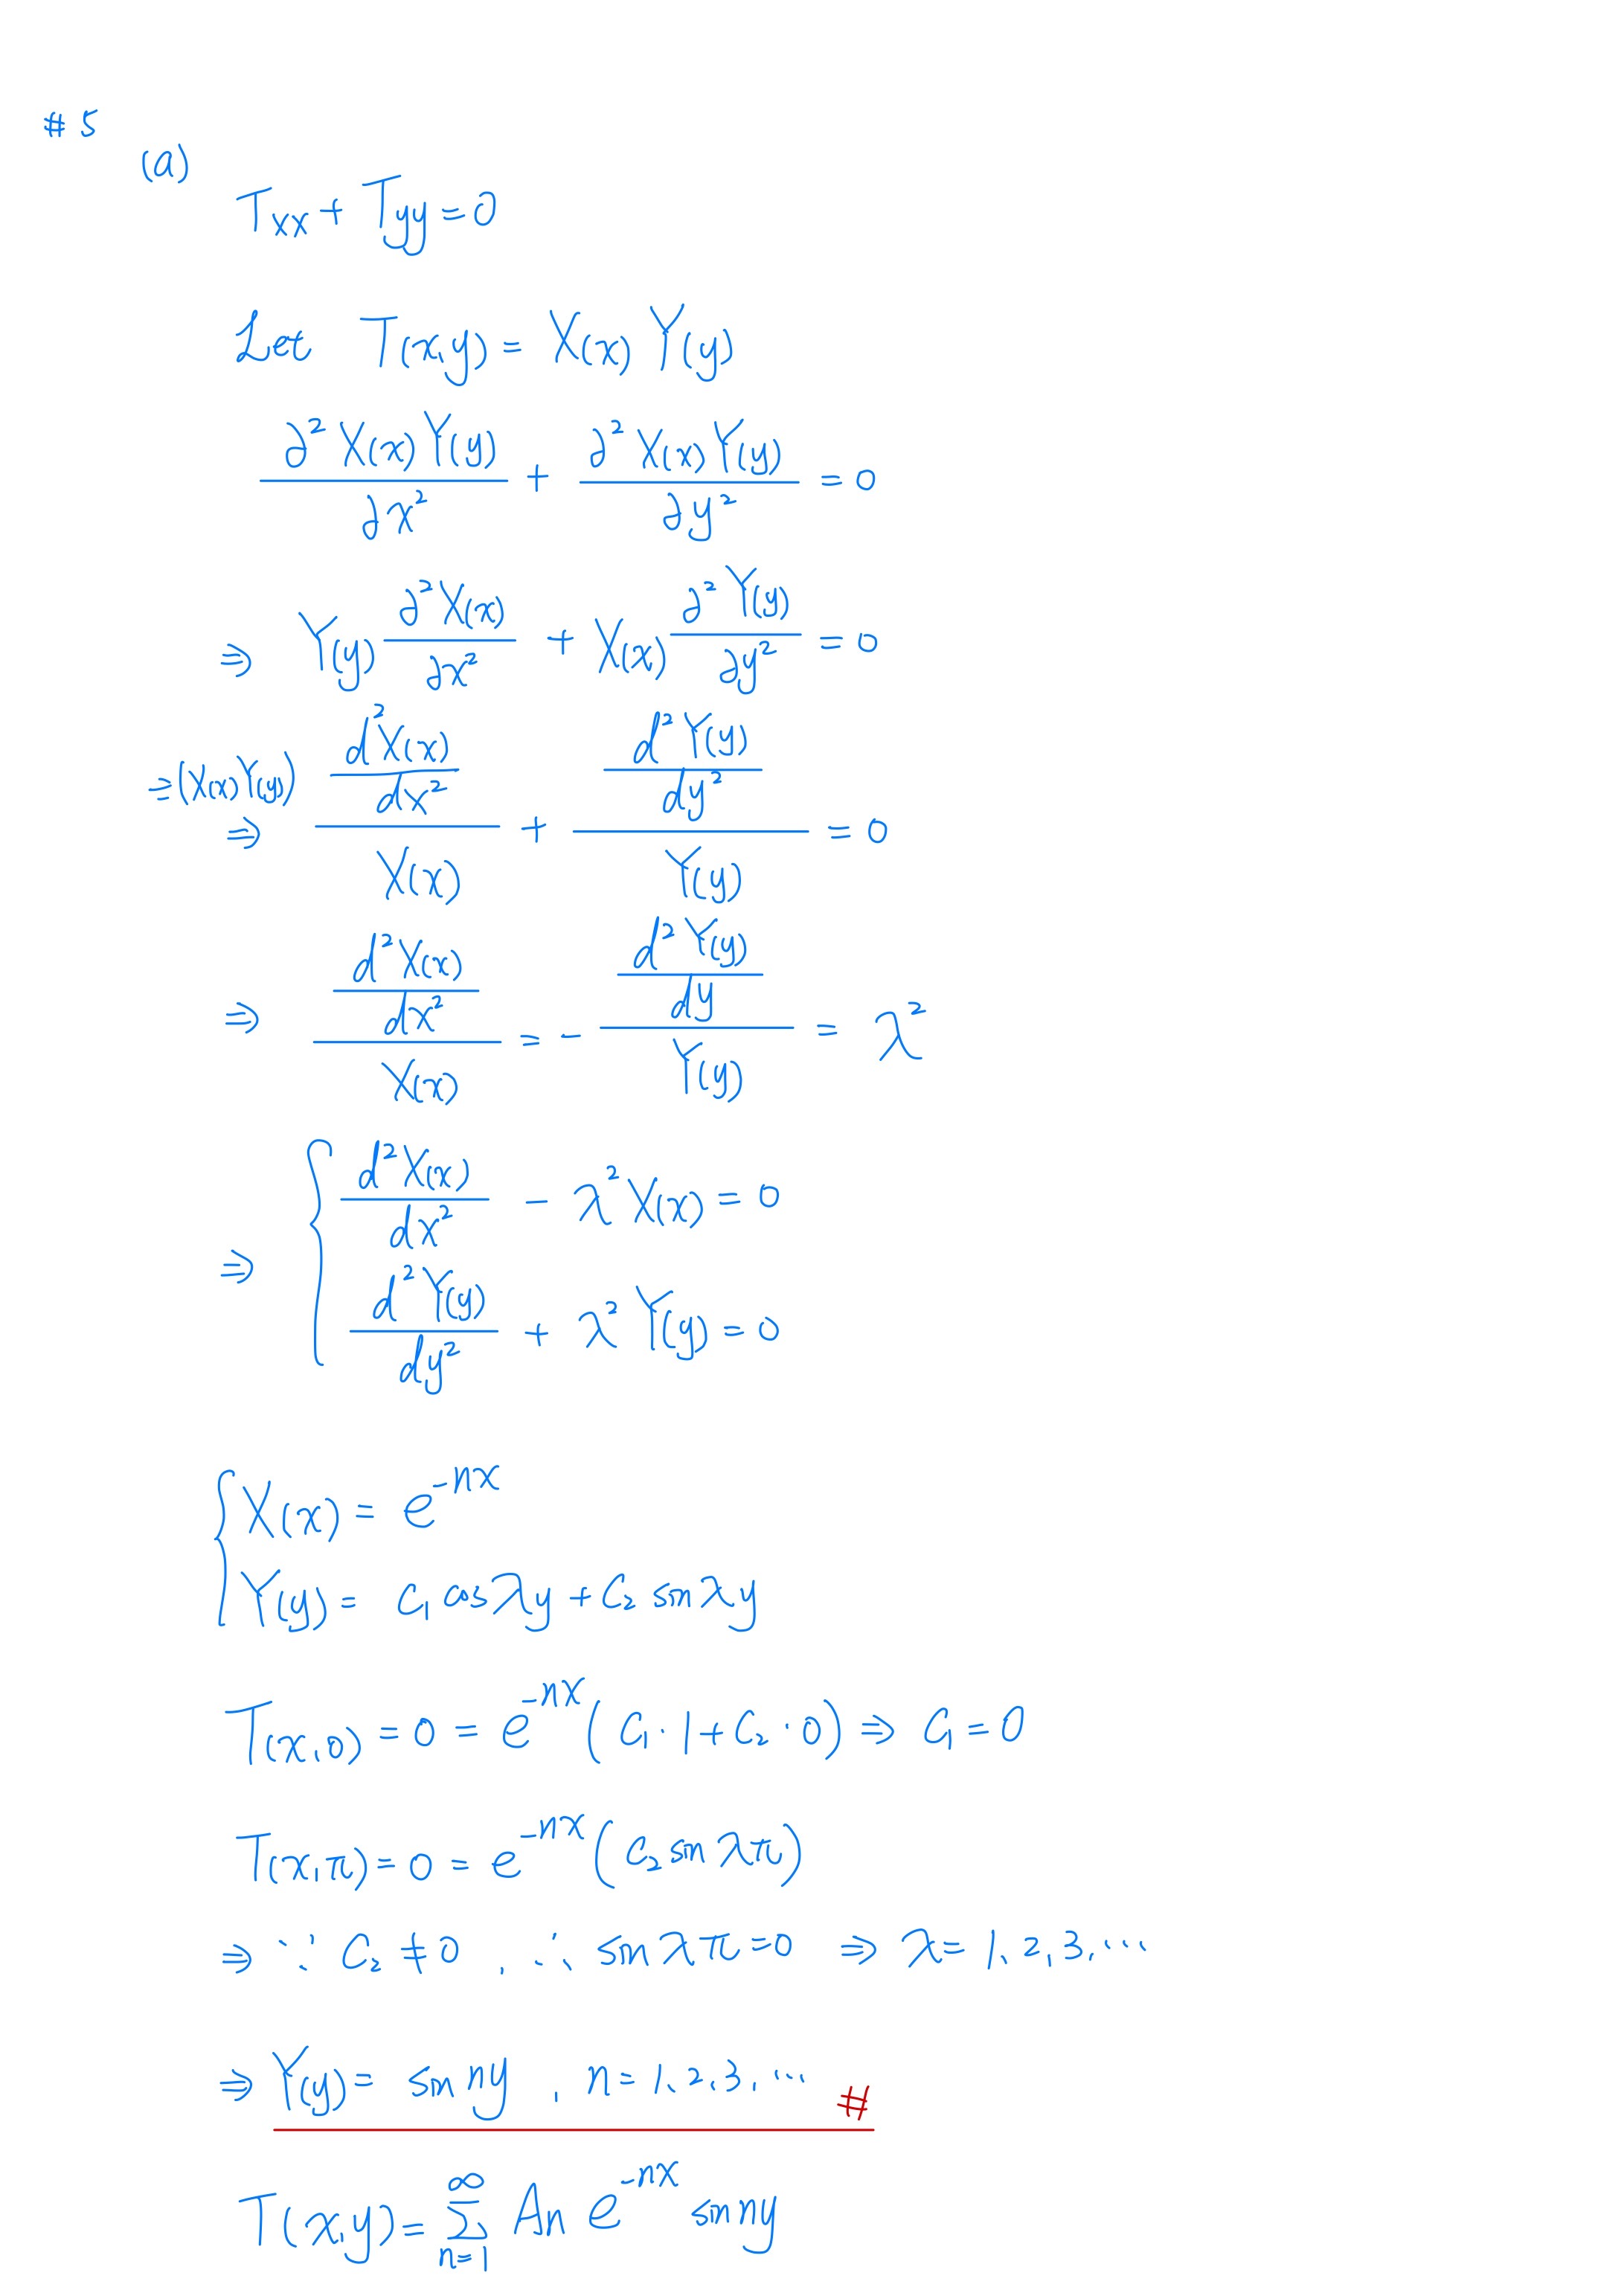
\includegraphics[width=6in, height=6.7in]{5(a)_1.jpg}
\newpage
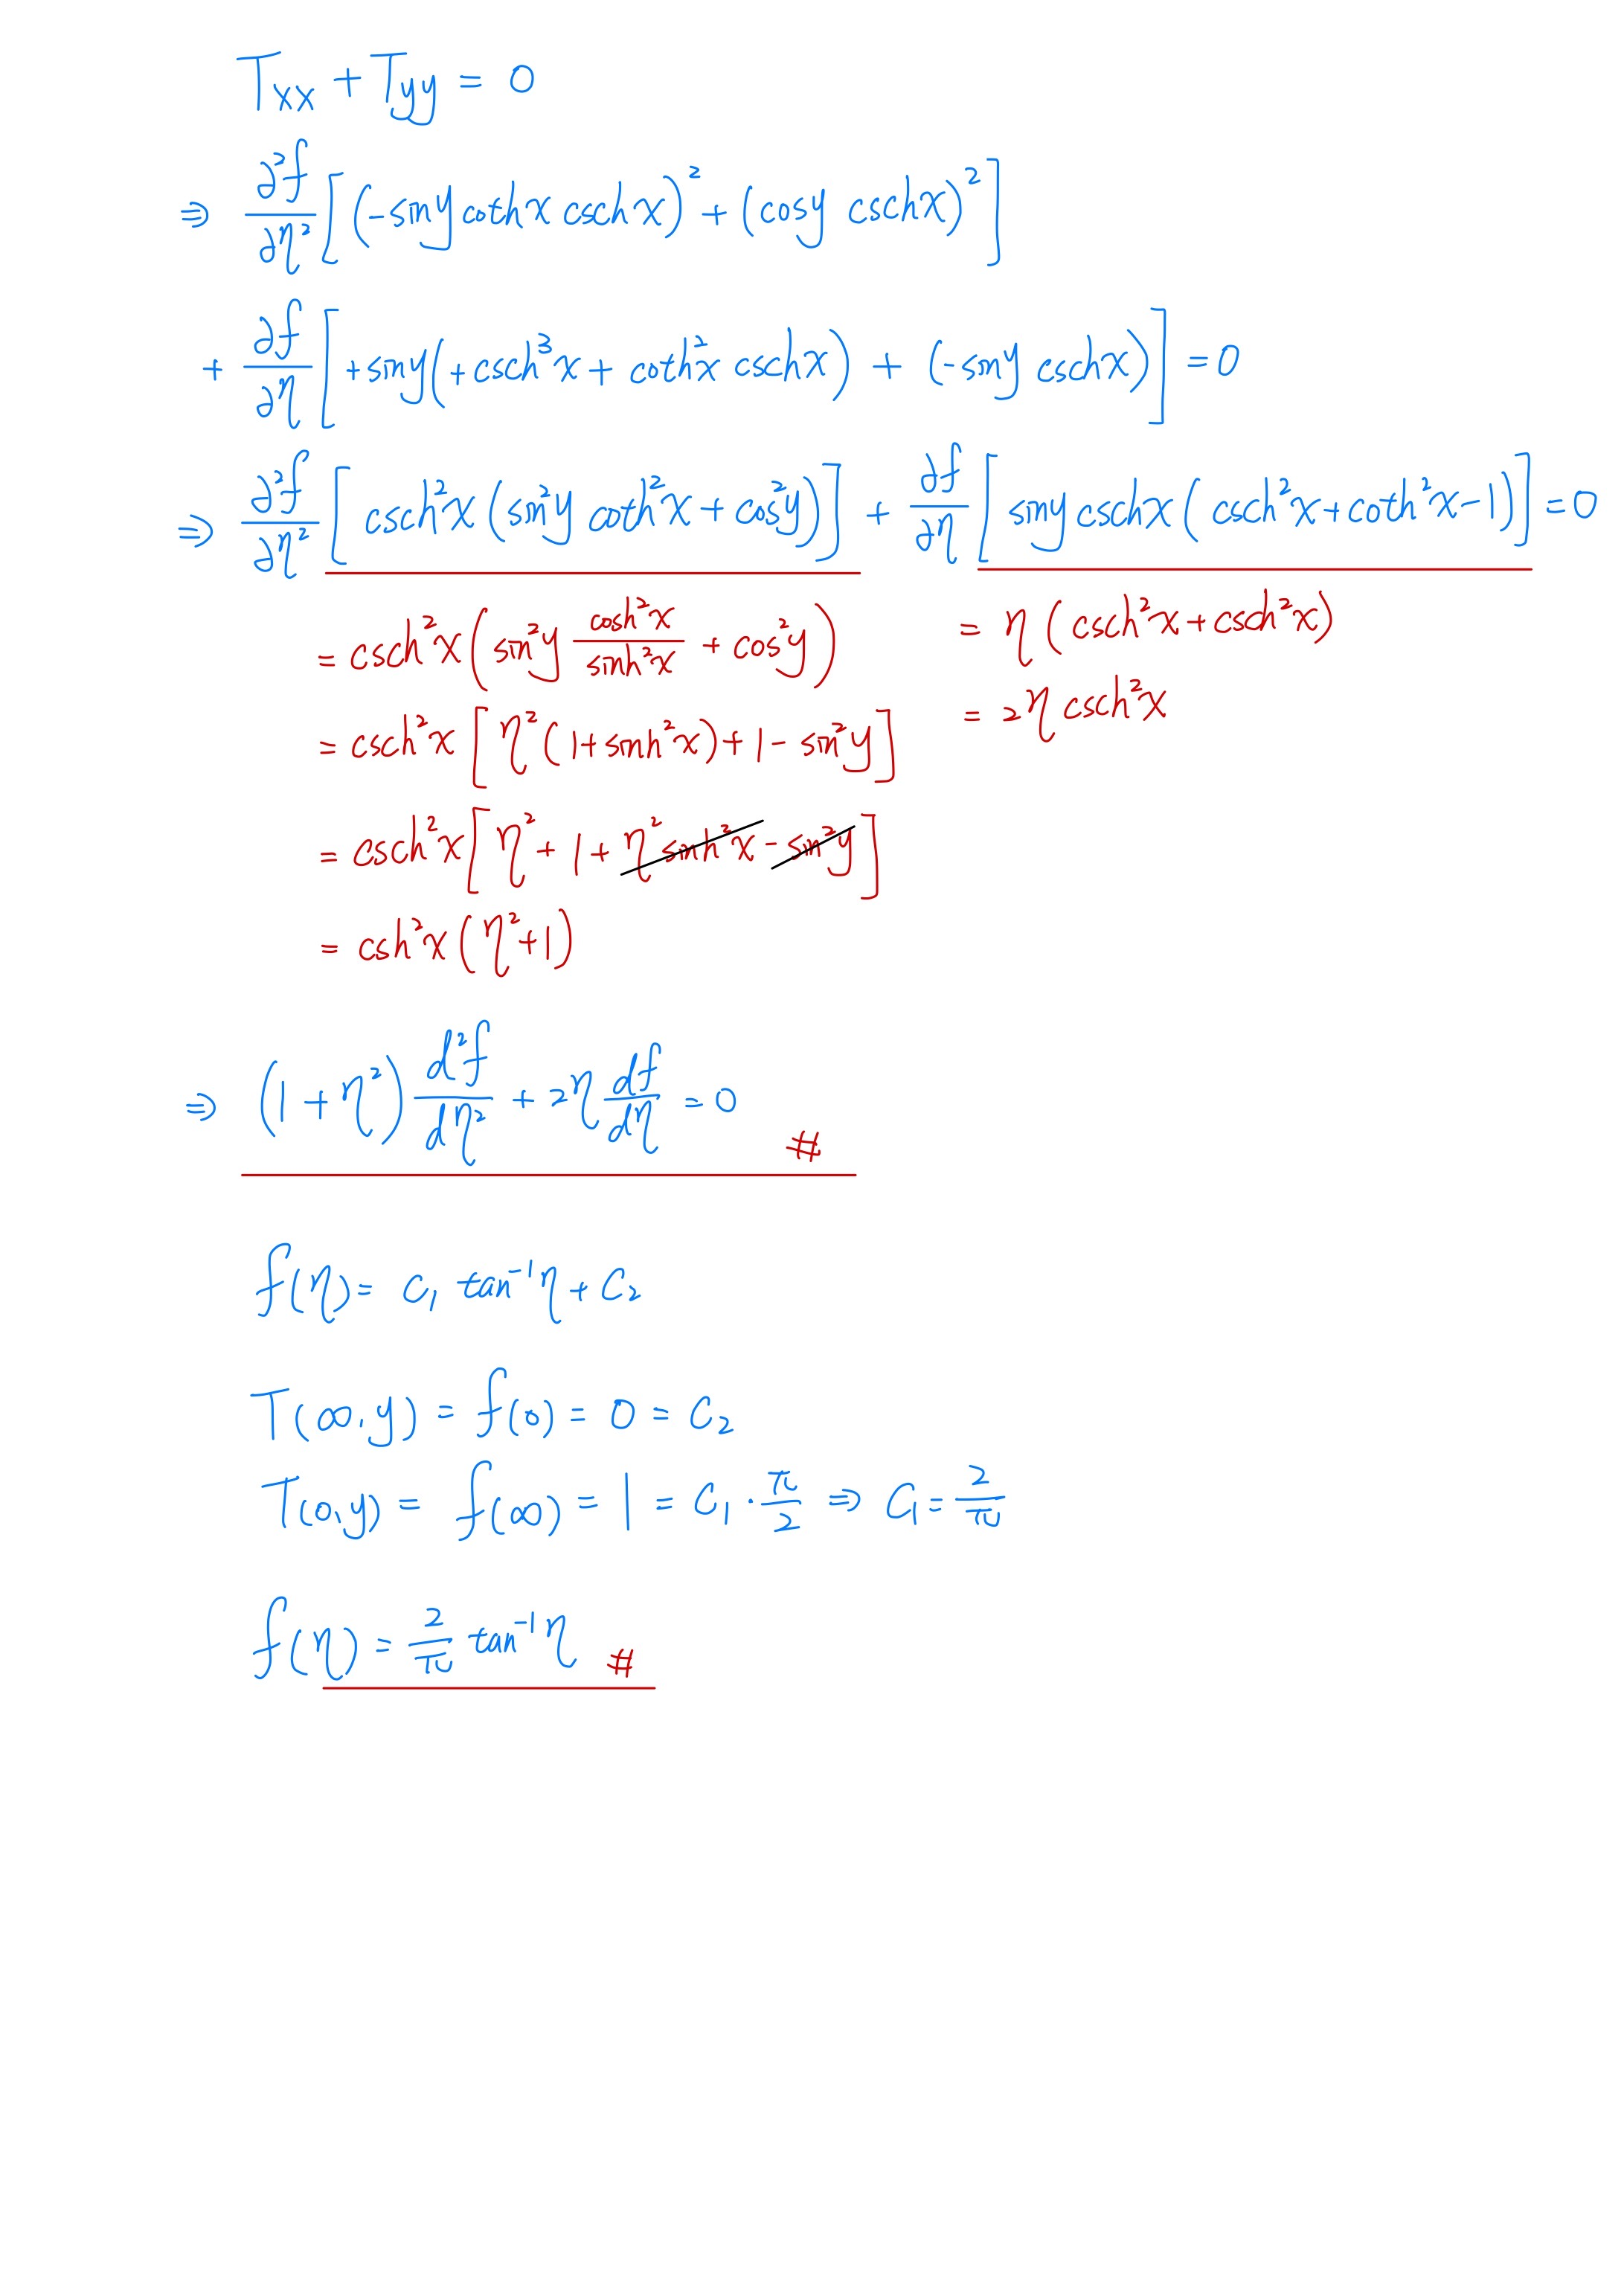
\includegraphics[width=6in]{5(a)_2.jpg}
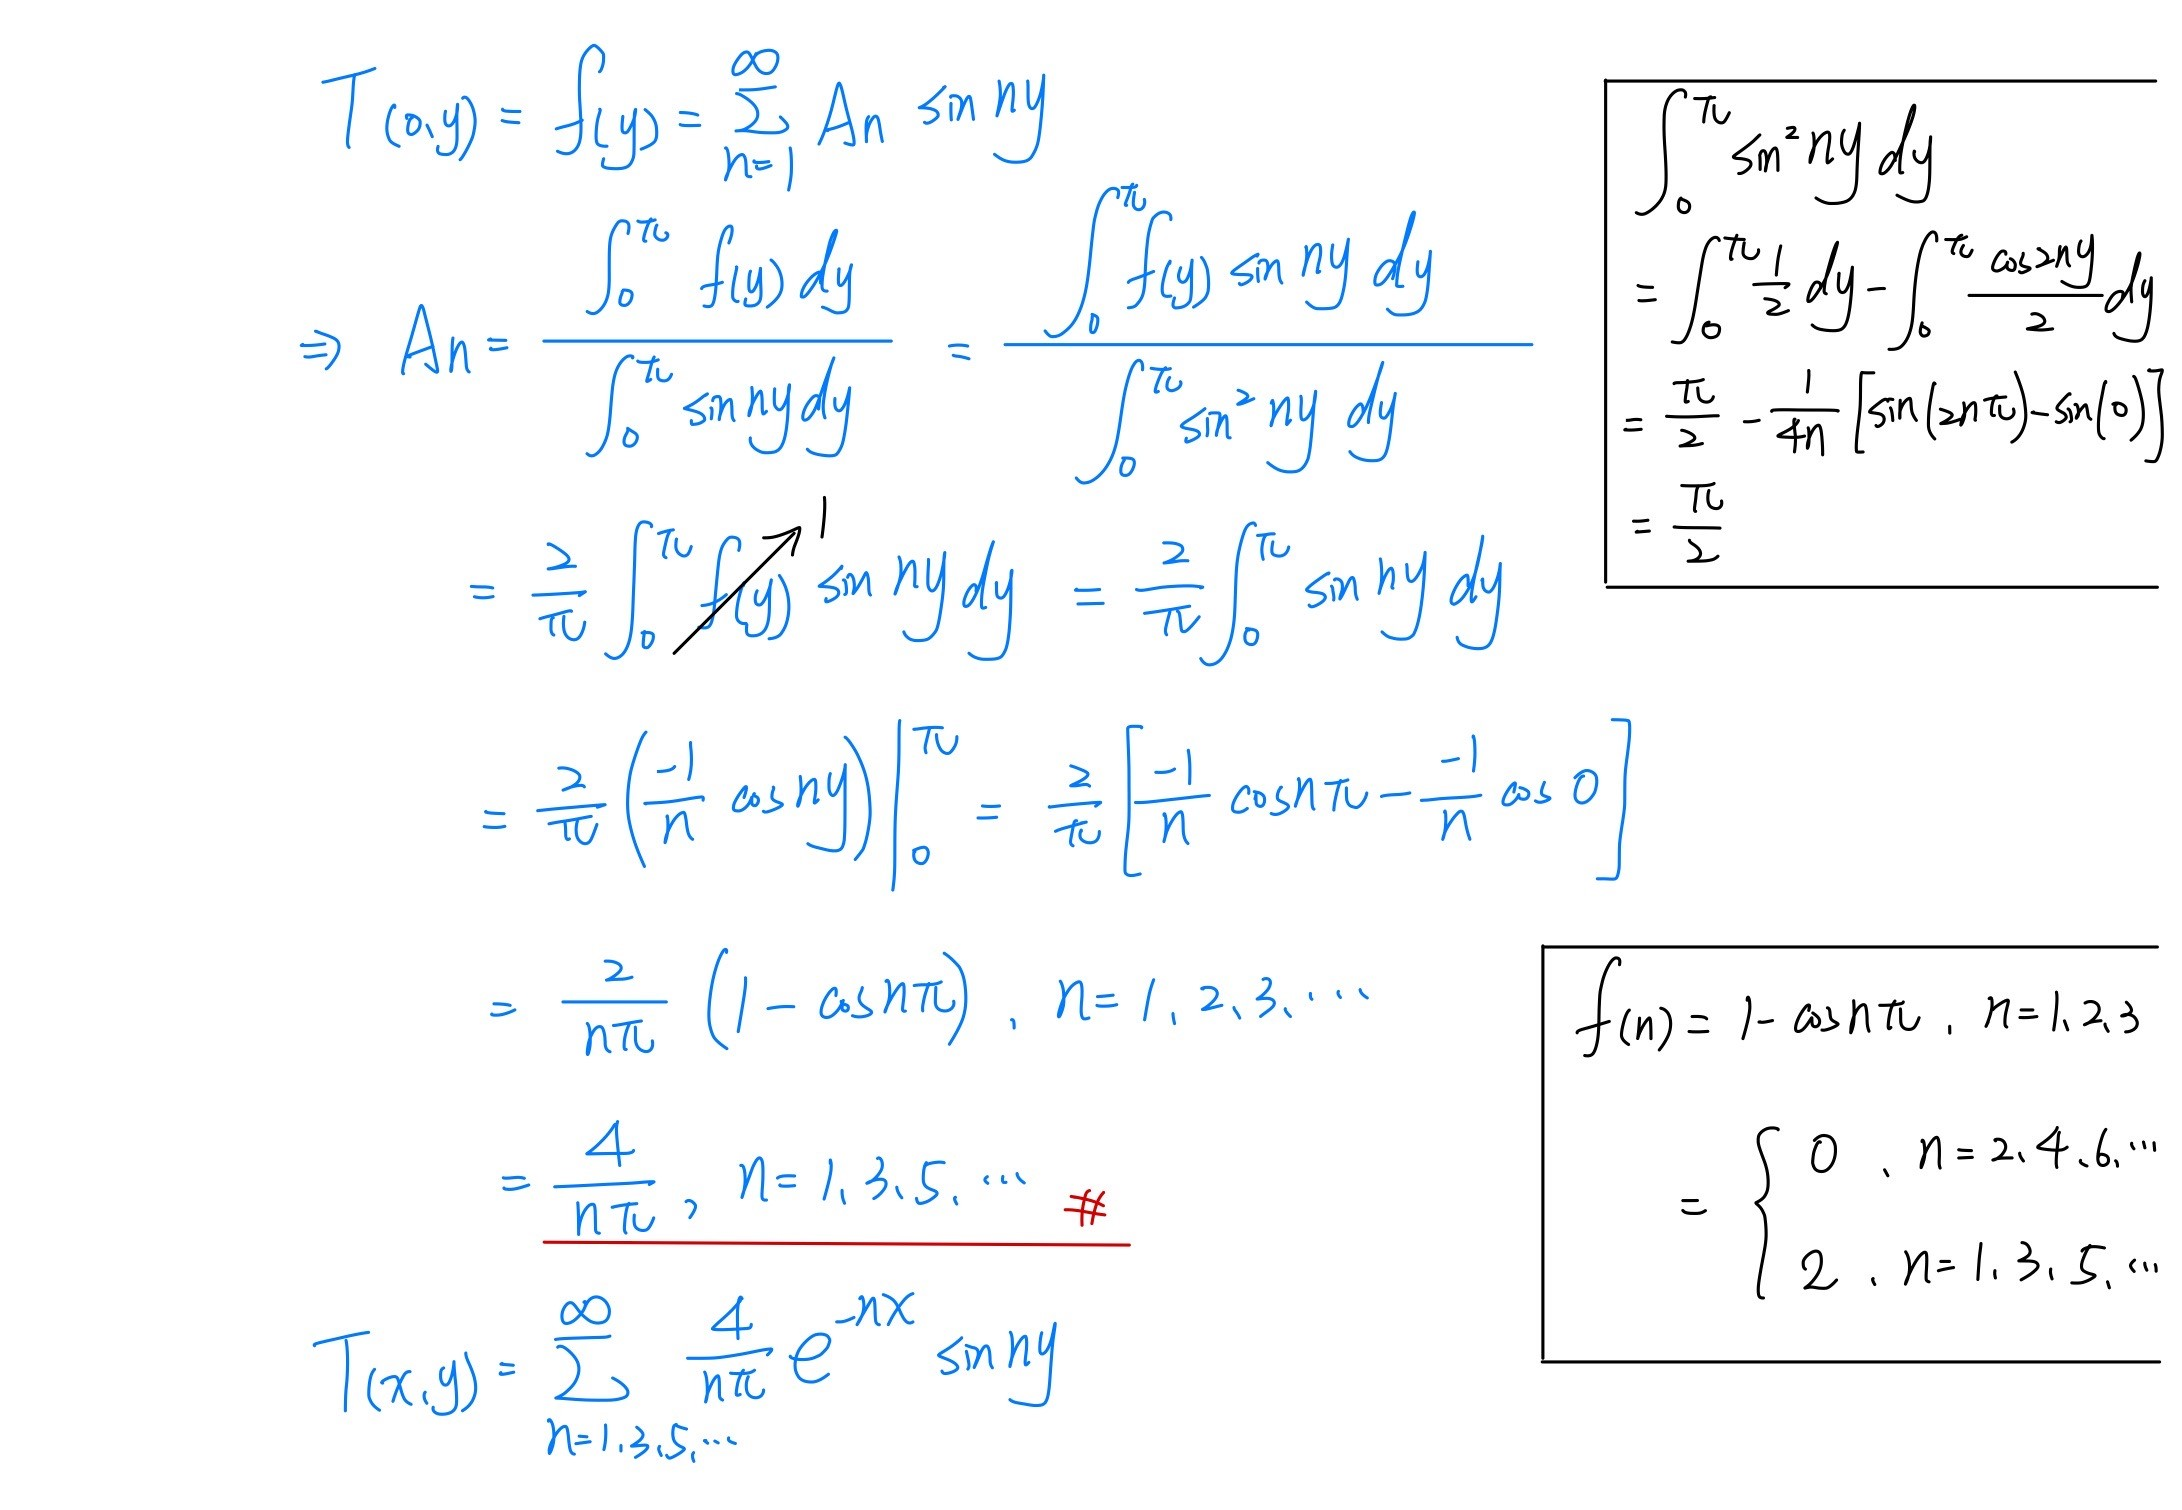
\includegraphics[width=6in]{5(a)_3.jpg}

\begin{verbatim}
clear;clc;close all
[x, y] = meshgrid(0:0.1:10,0:0.1:pi());
len = size(x);
for i = 1:len(1)
    for j = 1:len(2)
        f = @(n) exp(-(2.*n-1).*x(i,j)).*sin((2.*n-1).*y(i,j))./(2.*n-1);
        T(i,j) = 4/pi()*limsum(f,0);
    end
end
figure()
surf(x,y,T)
title("$\frac{4}{\pi}\sum_{n=1,3,5,...}^{\infty}\frac{1}{n}\exp^{-nx}\sin{ny}$ 3D Plot",...
'FontSize',15,'interpreter','latex')

figure()
contour(x,y,T,[.1 .3 .5],'ShowText','on')
title("$\frac{4}{\pi}\sum_{n=1,3,5,...}^{\infty}\frac{1}{n}\exp^{-nx}\sin{ny}$ 2D Plot",...
'FontSize',15,'interpreter','latex')
\end{verbatim}

\dotfill\\
\begin{multicols}{2}
    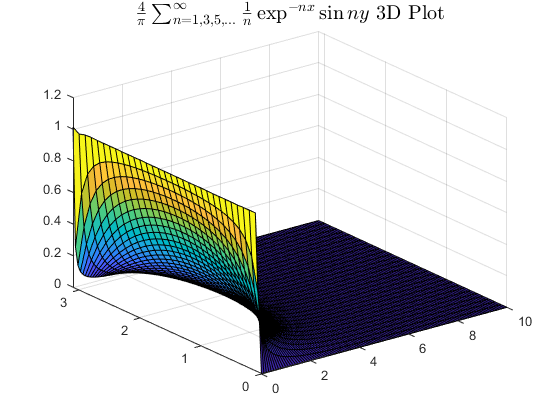
\includegraphics [width=3in]{HW1_17.png}

    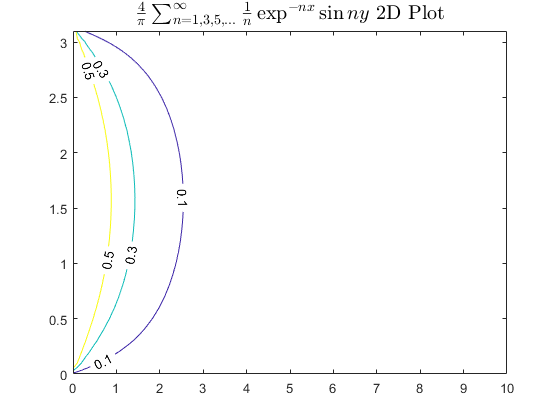
\includegraphics [width=3in]{HW1_18.png}
\end{multicols}

%-----------------------------------------
\hrulefill
\subsection*{\#5(b)}

\begin{verbatim}
clear;clc;close all
[x, y] = meshgrid(0:0.1:10,0:0.1:pi());
T = 2./pi().*atan2(sin(y),sinh(x));
figure()
surf(x,y,T)
title("$\frac{2}{\pi}\tan^{-1}{(\frac{\sin{y}}{\sinh{x}})}$ 3D Plot",...
'FontSize',15,'interpreter','latex')

figure()
contour(x,y,T,[.1 .3 .5],'ShowText','on')
title("$\ln(x^2+y^2)$ 2D Plot",'FontSize',15,'interpreter','latex')
\end{verbatim}

\dotfill\\
\begin{multicols}{2}
    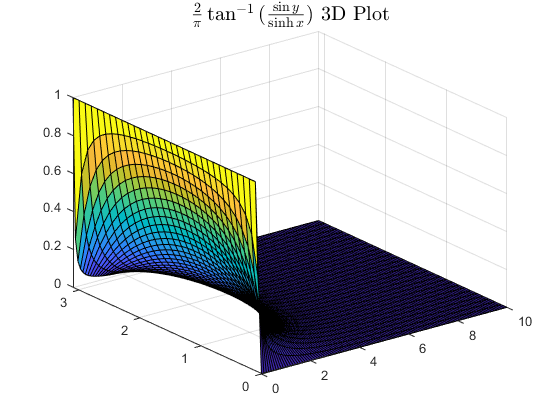
\includegraphics [width=3in]{HW1_19.png}

    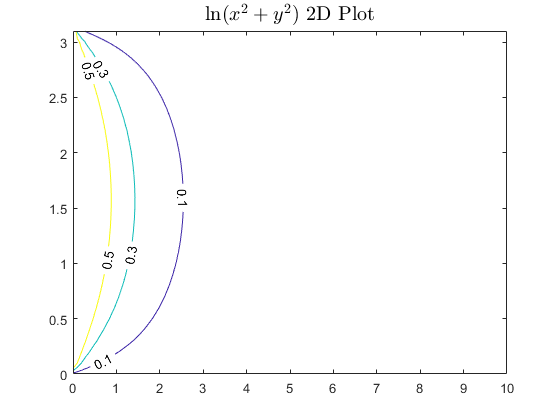
\includegraphics [width=3in]{HW1_20.png}
\end{multicols}

%=========================================
\hrulefill
\subsection*{function of \#1}

\begin{verbatim}
function sum = limsum(f,output)
    sum = 0;
    n = 1;
    while 1
        error = f(n);
        sum = sum + error;
        if abs(error) < 1e-6
            break
        end
        n = n+1;
    end
    if output == 1
        fprintf("Iteration times: %d \nValue: %f \nError: %f\n\n", n, sum, error)
    end
end
\end{verbatim}

%-----------------------------------------
\hrulefill
\subsection*{function of \#4}

\begin{verbatim}
function dydt = vibration_eqn(t, y)
    global w0 omega
    dydt = [y(2); -w0^2*y(1)+cos(omega*t)];
end
\end{verbatim}


\end{document}

